\chapter[Referêncial Teórico]{Referencial Teórico}

Este capítulo apresentará o referencial necessário para entendimento do conteúdo técnico da solução e contexto do problema.

\section{Classificação de documentos}

Nas áreas de NLP, existem grupos de técnicas para lidar com documentos de texto, assim como em ML. Destas, serão abordados apenas os conjuntos para a classificação de corpos de textos.

\subsection{Técnicas de pré-processamento}
As técnicas de pré-processamento utilizadas para a classificação de textos são as de transformação do texto em símbolos, remoção de palavras recorrentes, a radicalização, normalização e criação de regras específicas para cada contexto utilizando de expressões regulares \cite{oliveira_automatic_2017}.

\subsubsection{Transformação em símbolos}

A transformação em símbolos, trata-se de criar símbolos das palavras identificadas no texto \cite{manning_introduction_2008}.
A complexidade de como transformar a sentença numa lista de símbolos vai depender do contexto. Pode-se transformar endereços de rede, recursos de \textit{web site} em representações únicas \cite{manning_introduction_2008}. Na Tabela \ref{tab:palavrasSimbolos} é apresentado a separação da sentença em símbolos.

\begin{table}[ht]
	\centering    
	\caption[Transformação de palavras em símbolos]{Transformação de palavras em símbolos.}
    \label{tab:palavrasSimbolos}
	\begin{tabular}{|p{7cm}|p{7cm}|}
    \hline
    \textbf{Original} & \textbf{Símbolos textuais}\\ \hline
	juiz federal relator formar incisar iii \textbf{lei nº 11419} dezembro resolução trf região março conferência autenticidade documento disponível endereçar eletrônico \textbf{www.stf.org.br} & "juiz", "federal", "relator", "formar", "incisar", "iii", \textbf{"LEI\_11419"}, "dezembro", "resolução", "trf", "região", "março", "conferência", "autenticidade", "documento", "disponível", "endereçar", "eletrônico", \textbf{"SITE"}
    \\ \hline
    \end{tabular}\par Fonte: elaboração própria.
\end{table}

\subsubsection{Remoção de palavras recorrentes}

Ocorre, em documentos de texto, a repetição de algumas palavras que não trazem valor na classificação dos documentos. Essas podem ser removidas do texto, com isto diminui-se a quantidade de dados a serem processadas sem perder propriedades estatísticas e semânticas do texto \cite{manning_introduction_2008}. 

Na Tabela \ref{tab:palavrasRecorrentes} é apresentado a remoção das palavras: da, de, a, está.

\begin{table}[ht]
	\centering    
	\caption[Remoção de palavras recorrentes]{Remoção de palavras recorrentes.}
    \label{tab:palavrasRecorrentes}
	\begin{tabular}{|p{7cm}|p{7cm}|}
    \hline
    \textbf{Original} & \textbf{Palavras removidas}\\ \hline
	juiz federal relator forma inciso iii \textbf{da} LEI\_11419 \textbf{de de} dezembro resolução trf região março \textbf{a} conferência autenticidade documento \textbf{está} disponível endereço eletrônico SITE & juiz federal relator forma inciso iii LEI\_11419 dezembro resolução trf região março conferência autenticidade documento disponível endereço eletrônico SITE
    \\ \hline
    \end{tabular}\par Fonte: elaboração própria.
\end{table}

\subsubsection{Radicalização e Normalização}

Estas técnicas auxiliam na classificação dos textos, pois ressaltam propriedades estatísticas de uma palavra no texto. A tarefa de radicalização é remover sufixos e prefixos, verificar palavras compostas e substituí-las apenas pelo seu radical. Já a normalização, é transformar palavras que tenham diferentes formas com o mesmo significado para uma única representação \cite{singh_text_2016}. A Tabela \ref{tab:radicalizacaoNormalizacao} apresenta um exemplo de aplicação destas técnicas.

\begin{table}[ht]
	\centering    
	\caption[Aplicação de radicalização e normalização]{Aplicação de radicalização e normalização.}
    \label{tab:radicalizacaoNormalizacao}
	\begin{tabular}{|p{4cm}|p{4cm}|p{6cm}|}
    \hline
    \textbf{Original} & \textbf{Normalizado} & \textbf{Normalizado e Radicalizado} \\ \hline
	juiz federal relator \textbf{forma} \textbf{inciso} iii da LEI\_11419 de de dezembro resolução trf região março a conferência autenticidade documento \textbf{está} disponível endereço eletrônico SITE & juiz federal relator \textbf{formar} \textbf{incisar} iii da LEI\_11419 de de \textbf{dezembro} \textbf{resolução} trf região março o \textbf{conferência} autenticidade documento estar disponível endereçar eletrônico SITE & juiz federal relator form incis iii da lei\_11419 de de dezembr resolu trf regiã marc o conferent autent document estar dispon enderec eletrôn sit
    \\ \hline
    \end{tabular}\par  Fonte: elaboração própria.
\end{table}

\subsubsection{Expressões regulares}

Quando deseja-se encontrar algum padrão específico em um texto, utiliza-se de regras de formação para capturar todos os grupos que se encaixaram. Esta técnica também  auxilia a realizar substituições, remover trechos do texto. Ela diminui a complexidade de código para realizar manipulações em \textit{strings} \cite{goyvaerts_regular_2012}. A Tabela \ref{tab:regex} mostra um exemplo da aplicação das expressões regulares presentes no Apêndice \ref{sec:apendiceA}.

\begin{table}[ht]
	\centering    
	\caption[Aplicação de expressões regulares]{Aplicação de expressões regulares.}
    \label{tab:regex}
	\begin{tabular}{|p{7cm}|p{7.6cm}|}
    \hline
    \textbf{Original} & \textbf{Processado com Expressão Regular} \\ \hline
	Juiz Federal Relator, na\textbackslash nforma do artigo 1º , inciso III, da Lei 11.419, de 19 de dezembro de 2006 e Resolução TRF 4ª\textbackslash nRegião nº 17, de 26 de março de 2010. A conferência da autenticidade do documento está\textbackslash ndisponível no endereço eletrônico http://www.jfpr.jus.br/ gedpro/verifica/verifica.php, & juiz federal relator forma inciso iii da LEI\_11419 de de dezembro resolução trf região março a conferência autenticidade document está disponível endereço eletrônico SITE \\ \hline
    \end{tabular}\par  Fonte: elaboração própria.
\end{table}

\subsection{Representações de textos}

Quando faz-se o processamento de linguagem natural, utiliza-se diferentes formas de representação para o texto ao invés de \textit{string}. As técnicas utilizadas são as de \textit{one-hot-encoder}, \textit{bag of words} (BoW) e \textit{word embedding}.

\subsubsection{One-hot-encoder}

Esta técnica consiste em transformar cada palavra num único vetor, no qual a posição da palavra no dicionário de dados receberá o valor 1. Desta forma, uma sentença se tornará uma matriz, como no exemplo abaixo \cite{brink_real-world_2015}.

\begin{center}
    $
    \begin{array}{rcccc}
        Frase = & [ 0 & 1 & 0 & 0 ]  \\
        de  = & [ 1 & 0 & 0 & 0 ]  \\
        exemplo = & [ 0 & 0 & 1 & 0 ]  \\
        simples = & [ 0 & 0 & 0 & 1 ]  \\
    \end{array}
  	$
\end{center}

\subsubsection{Bag of Words - BoW}

Diferentemente do \textit{One-hot-encoder}, o BoW transforma toda a sentença em apenas um vetor. Cada posição deste, possuirá a quantidade de vezes que um símbolo apareceu. Ela permite que possam ser removidas palavras com alta ou baixa incidência \cite{brink_real-world_2015}.

\begin{center}
    $
    \begin{array}{rccccc}
        \label{ex:bow}
        Frase\ de\ exemplo\ simples = & [ 1 & 1 & 1 & 1 & 0]  \\
        Frase\ de\ frase\ repetida = & [ 2 & 1 & 1 & 0 & 1]  \\
    \end{array}
  	$
\end{center}

% \subsubsection{Word Embedding}

% O \textit{word embedding}, diferentemente dos métodos anteriores que são representados como símbolos únicos, lida com uma representação distribuída \cite{goldberg_neural_2017}.

% Neste método, o significado de uma palavra, que foi capturada numa janela de contexto, é representado na forma de um vetor. Cada dimensão deste vetor não representa necessariamente um aspecto do mundo real, mas o conjunto delas que trás alguma significância \cite{goldberg_neural_2017}. Entende-se as palavras como vetores que podem possuir relações em seu espaço de representação, como na Figura \ref{fig:wordtovec}. 

% \begin{figure}[h]
% 	\centering
% 	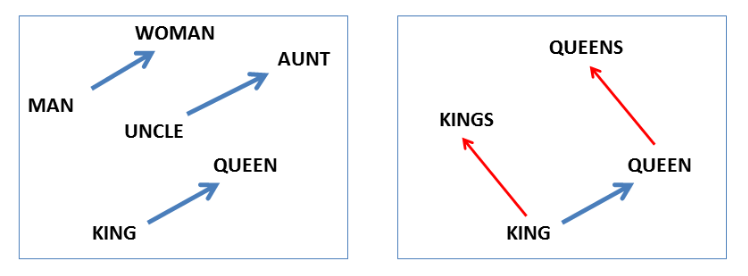
\includegraphics[keepaspectratio=true,scale=0.5]{figuras/wordtovec}
%     \caption[Representação discreta de palavras]{Representação discreta de palavras. Fonte: \cite[Página 479]{mikolov_linguistic_2013}.}
%     \label{fig:wordtovec}
% \end{figure}
% Com os vetores das palavras Rei, Rainha, Homem e Mulher torna-se possível realizar consultas às palavras da forma: $vect('Rei') + vect('Mulher') - vect('Homem')$, no qual a resposta é Rainha \cite{mikolov_linguistic_2013}. Esta proposição também se confirma para outras relações como País-Capital e Adjetivos Aumentativo-Diminutivo \cite{mikolov_distributed_2013}.

% \begin{center}
%     $
%     \begin{array}{rlrrrrr}
%         \label{ex:we}
%         Palavra = & [ & Sexo & Realeza & Pluralidade & Parentesco &] \\ \hline
%         Rei = & [ & 1 & 1 & -1 & 0,5 & ]  \\
% 		Reis = & [ & 1 & 1 & 1 & 0,5 & ]  \\
%         Rainha = & [ & -1 & 1 & -1 & 0,5 & ] \\
%         Rainhas = & [ & -1 & 1 & 1 & 0,5 & ] \\
%         Homem = & [ & 1 & 0 & -1 & 0 & ] \\
%         Mulher = & [ & -1 & 0 & -1 & 0 & ] \\
%         Tio = & [ & -1 & 0 & -1 & 1 & ] \\
%         Tia = & [ & 1 & 0 & -1 & 1 & ] \\
%     \end{array}
%   	$
% \end{center}

% No exemplo acima, cada palavra é representada por um vetor, no qual, foram definidas apenas quatro dimensões de exemplos. As duas principais formas de chegar a este resultado é pelo \textit{Word2Vect} elaborado por \citeauthor{mikolov_distributed_2013} (\citeyear{mikolov_distributed_2013}) e o \textit{GloVe} definido por \citeauthor{pennington_glove:_2014} (\citeyear{pennington_glove:_2014}).

% O uso de \textit{word embedding} para modelos de classificação, são mais estáveis \cite{enriquez_approach_2016}, representam ganhos de acurácia para classificação de textos curtos \cite{butnaru_image_2017} \cite{ge_improving_2017}.

\subsection{Técnicas de ML}

As principais técnicas para aprendizado de máquina para classificação de texto são Máquinas de Vetores de Suporte (do inglês \textit{Suporte Vector Machine} SVM), K Vizinhos Próximos, Multinomial Naive Bayes.

Para este trabalho, utiliza-se apenas o modelo SVM. Isto porque serve para lidar com vetores que possuem muitas características. Além disso, seu algoritmo possibilita extrair dos vetores de suporte, os quais são as dimensões mais importantes para realizar a separabilidade dos dados \cite{hearst_support_1998} e possui boa performace para classificar corpos textuais maiores \cite{wang_baselines_2012}.

\subsubsection{Máquinas de Vetores de Suporte}

Este algoritmo recebe os vetores de entrada, com uma alta dimensionalidade, e faz transformações neles utilizando seus núcleos para que seja possível aplicar métodos lineares, mesmo em problemas não-lineares \cite{hearst_support_1998}.

\begin{figure}[ht]
	\centering
    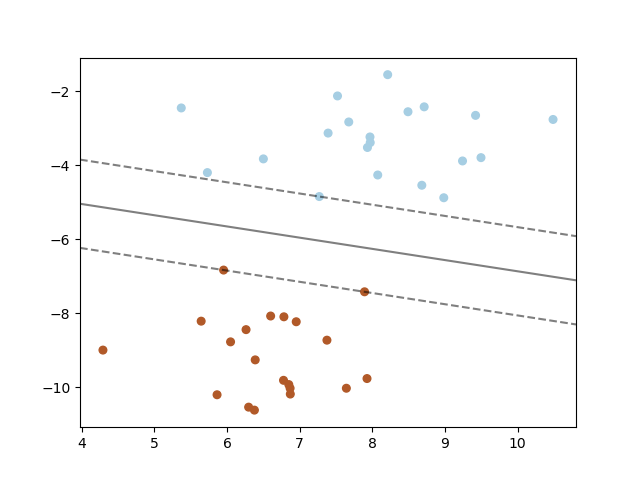
\includegraphics[keepaspectratio=true,scale=0.7]{figuras/svmExample}
	\caption[SVM Funcionamento]{Funcionamento do algoritmo SVM. Fonte: \citeonline[Acesso em 10 de Junho de 2018.]{pedregosa_scikit-learn:_2011}}
	\label{fig:svmExample}
\end{figure}

A função de classificação do SVM é baseada em hiperplanos. O algoritmo busca otimiza-los de forma que ele fique ortogonal às linhas que separam as duas classes, como é possível ver na Figura \ref{fig:svmExample}. Chama-se estes vetores de separação de suporte \cite{smola_tutorial_2004}.

\begin{equation} \label{eq:svmFormula}
	f(x) = sign(\sum_{i=1}^{t} v_i \cdot k(x, x_i) + b)
\end{equation}

A Equação \ref{eq:svmFormula} é a de classificação utilizada neste algoritmo. A função $k$ é a que representa o núcleo, na implementação de \citeonline{pedregosa_scikit-learn:_2011} existe disponível o: linear, polinomial, função de base radial (do inglês \textit{Radial Basis Function} RBF) e o de sigmoide.

O valor de $x$ em \ref{eq:svmFormula} representa o vetor de entrada a ser classificado. Já o $x_{i}$ representa os vetores de suporte. Os pesos $v_{i}$, são calculados através de uma solução quadrática, no qual são a combinação linear dos padrões de entrada \cite{smola_tutorial_2004}. Os valores de $b$, são limiares para maximização das margens entre duas classes distintas \cite{hearst_support_1998}.

\subsubsection{Redes neurais}

Um dos algoritmos desenvolvidos para realizar o aprendizado de máquina, foi baseado em um neurônio humano \cite{goldberg_neural_2017}. O neurônio, chamado de perceptron possui sensores de retina (entrada), os sinais recebidos se propagam para uma área de associação, onde são combinados. O sinal propagado para as ligações a frente, se e apenas se, o valor dele for maior que um limitar $\theta$ \cite{raschka_single-layer_2015}.

Como na figura \ref{fig:perceptron}, há pesos para os vetores de entrada, que são todos somados e, em seguida, passam pela função de ativação para gerar o resultado do perceptron \cite{raschka_single-layer_2015}. 

\begin{figure}[ht]
	\centering
    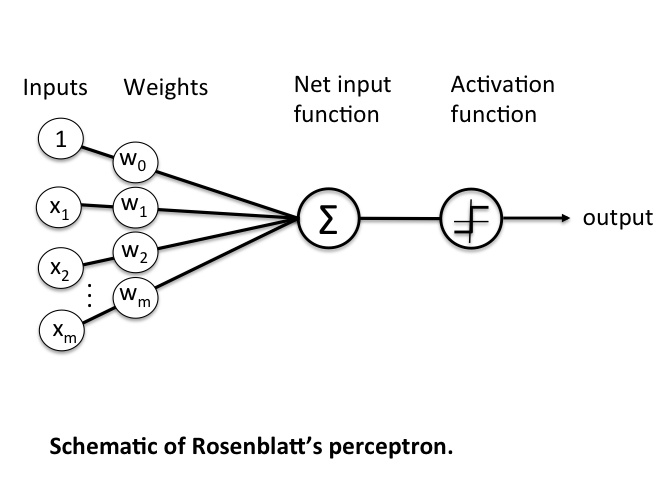
\includegraphics[keepaspectratio=true,scale=0.5]{figuras/perceptronSchematic}
	\caption[Ilustração Perceptron]{Ilustração esquemática de um perceptron de Rosenblatt. Fonte: 
\citeonline[Acesso em 10 de Junho de 2018]{raschka_single-layer_2015}.}
	\label{fig:perceptron}
\end{figure}

Agrupou-se os neurônios para criar uma rede, na qual ela possui diferentes camadas.

\begin{description}
	\item \textbf{Entrada}: esta camada não possui funções de ativação, sua função é propagar os dados de entrada para a camada seguinte.
    \item \textbf{Camadas ocultas}: são as camadas que possuem funções de ativações. Uma camada oculta pode possuir vários neurônios.
    \item \textbf{Saída}: esta é a ultima camada de uma rede neural, ela que irá retornar o resultado do processamento realizado pelas camadas ocultas.
\end{description}

\begin{figure}[ht]
	\centering
    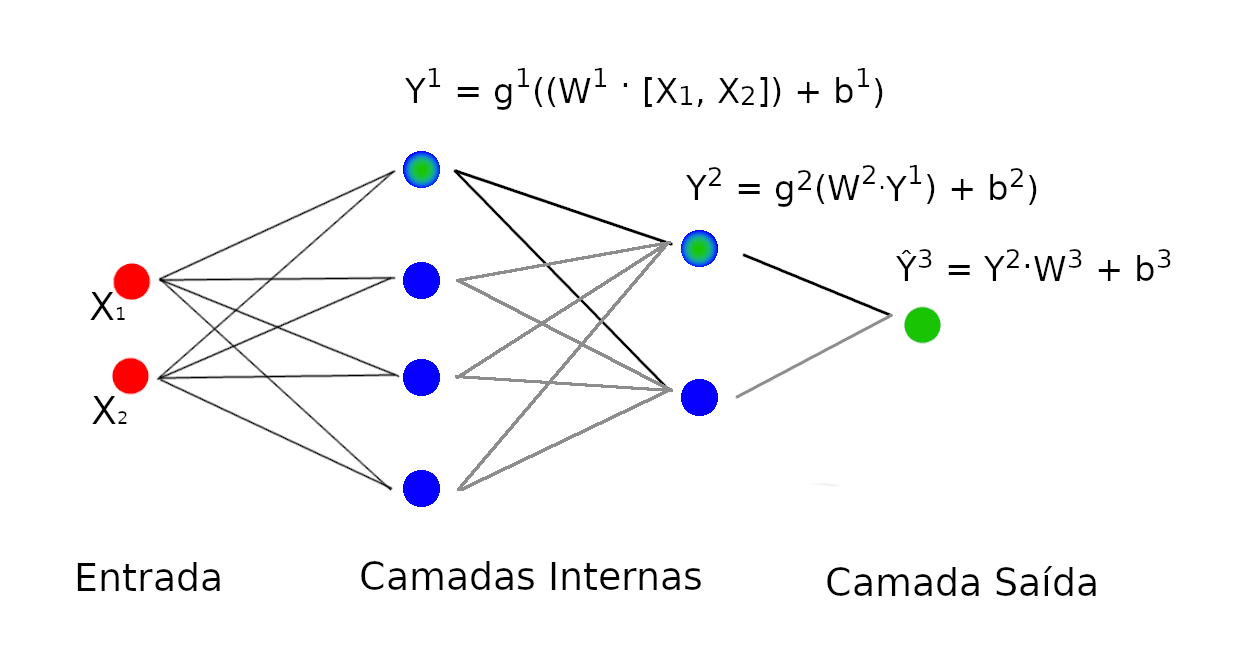
\includegraphics[keepaspectratio=true,scale=1.3]{figuras/redeNeural}
	\caption[Rede Neural Simples]{Representação de uma rede neural com duas camadas internas, dois neurônios de entrada e apenas um de saída. Fonte: elaboração própria}
	\label{fig:redeNeural}
\end{figure}

Os neurônios com a coloração verde na figura \ref{fig:redeNeural}, indicam que apenas estes foram ativados durante o processamento.
 
O fluxo comum da execução de uma rede neural é o recebimento dos dados de entrada na primeira camada, em seguida há a propagação dos valores para uma camada oculta, após o cálculo de ativação, os dados são propagados novamente para a próxima camada, até que ao final, chega-se na camada de saída \cite{goldberg_neural_2017}.

O processo de propagação (do inglês \textit{feed-forward propagation}) é representado na Figura \ref{fig:redeNeural}, no qual há propagação dos valores com o produto entre o vetor $x$ e $W$ \cite{goldberg_neural_2017}. A representação de vetores da computação para os pesos são feitas de forma que o neurônio da camada seguinte $i$ tem o peso associado a posição $j$ ($W[i][j]$) \cite{nielsen_neural_2015}.

Para modelos com mais camadas do que foi ilustrado na Figura \ref{fig:redeNeural}, pode-se generalizar a equação lá apresentada. Em cada camada $i$, o vetor $W^{i}$ possui dimensão $d^{i}_{in} \times d^{i}_{out}$ dimensões. Os vetores de viés $b^{i}$ terão $1 \times d^{i}_{out}$. O valor de $N$ é igual ao número de camadas na rede. Na Equação \ref{eq:multilayer}, cada camada da rede neural poderá ter sua própria função de ativação \cite{goldberg_neural_2017}. 

\begin{displaymath}
    x^{i} = 
    \begin{cases}
      x & \textit{se for camada de entrada} \\
      \hat{y}^{i-1} & \textit{caso contrário} \\
    \end{cases}       
\end{displaymath}
\begin{equation}
	\label{eq:multilayer}
    y^{i} = g^{i}(x^{i}W^{i} + b^{i})
\end{equation}
\begin{displaymath}
    \hat{y} = y^{N-1}W^{N}
\end{displaymath}

Para ajustar os valores dos pesos e vetor de viés $W^{i}$ e $b^{i}$, calcula-se o quanto os neurônios estão corretos em relação ao distanciamento entre o $\hat{y}$ e $y$. Utiliza-se da função de erro $L(\hat{y}, y)$ \cite{goldberg_neural_2017}, para calcular o erro na camada de saída. Este deve ser propagado para a camada anterior, com isto, todas as camadas vão ajustando recursivamente seus pesos e vetores de viés \cite{nielsen_neural_2015}. Este processo chama-se de retro-propagação (do inglês \textit{back-propagation}) apresentado na Figura \ref{fig:redeNeuralBackprop}.

\begin{figure}[ht]
	\centering
    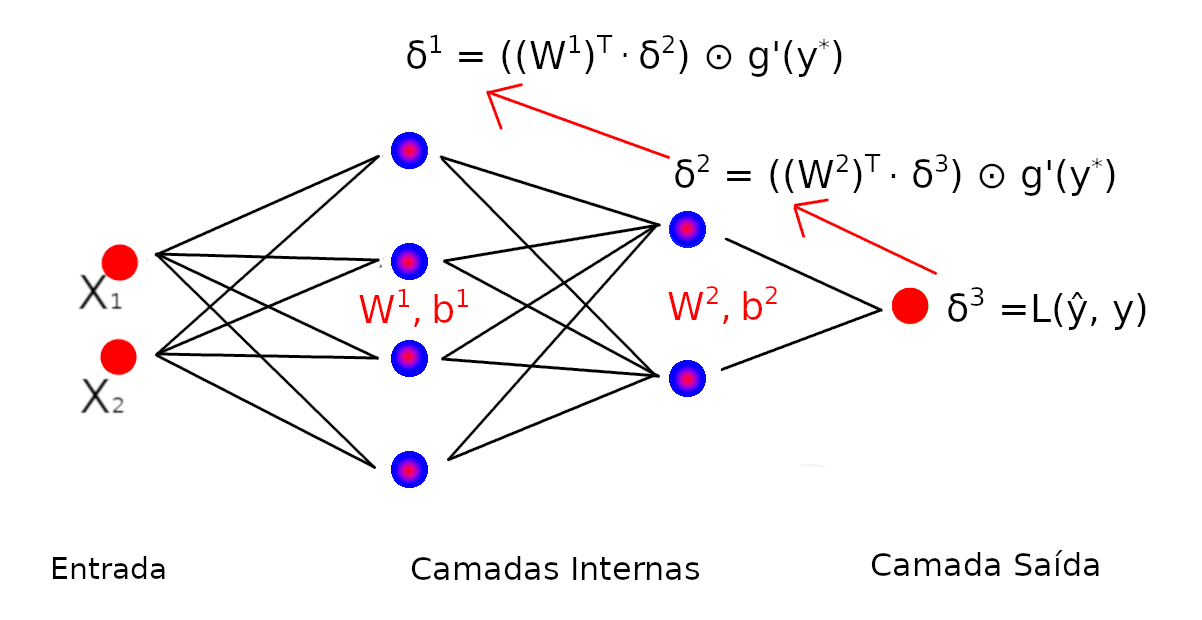
\includegraphics[keepaspectratio=true,scale=1.3]{figuras/redeNeuralBackprop}
	\caption[Retro-propagação em Rede Neural]{Simplificação da retro-propagação em Rede Neural. Fonte: elaboração própria}
	\label{fig:redeNeuralBackprop}
\end{figure}

Na Figura \ref{fig:redeNeuralBackprop}, o valor de $g'$ é a derivada para a função de ativação, executada no valor de $y^{*}$, o qual é o resultado da operação de $x^{i}W^{i} + b^{i}$ sem aplicar a função de ativação $g$ \cite{nielsen_neural_2015}.

A operação de $\bigodot$ é o produto de Hadamard, ela representa multiplicar os elementos de cada posição de um vetor $a_{n}$ pelo do valor de $b_{n}$ resultando em um outro vetor $c_{n}$ \cite{nielsen_neural_2015}. A Equação \ref{eq:hadamard} ilustra essa operação entre os vetores.

\begin{equation}
	\label{eq:hadamard}
	\begin{bmatrix}
    	3 \\
        7 \\
	\end{bmatrix}
    \bigodot
    \begin{bmatrix}
    	4 \\
        9 \\
	\end{bmatrix}
    =
    \begin{bmatrix}
       3 & * & 4 \\
       7 & * & 9 \\
    \end{bmatrix}
     =
    \begin{bmatrix}
    	12 \\
        63 \\
	\end{bmatrix}     
\end{equation}
Com a função de $\delta^{i}$, faz-se a atualização dos pesos e vetores de viés. A estrutura é recursiva, de forma que, para calcular o $\delta^{i}$, é necessário ter calculado o valor de $\delta^{i+1}$. A prova matemática para a retro-propagação e a definição da função $L(\hat{y}, y)$ encontra-se em \citeonline{nielsen_neural_2015}.

A retro-propagação é utilizada juntamente com uma função de gradiente. Com esta combinação, faz-se os ajustes nos pesos das camadas, de forma que, a cada nova predição de $\hat{y}$, é feita uma retro-propagação calculando os valores mínimos para a função $L(y, \hat{y})$ \cite{nielsen_neural_2015}.

Com as técnicas apresentadas, é possível implementar uma rede neral Multicamadas de Perceptron (do inglês \textit{Multilayer Perceptron} - MLP). Existem outros tipos de arquiteturas, como as Redes Neurais Recorrentes (RNN), as Redes Neurais Convolucionais (CNN). Elas podem ser utilizadas como camadas internas de uma MLP, bem como podem existir camadas de mescla (do inglês \textit{merge}) e de junção (do inglês \textit{pooling}) \cite{goldberg_neural_2017}.

\subsection{Técnicas de Aprendizado Profundo}

O aprendizado de máquina profundo é quando utiliza-se várias camadas ocultas em uma rede neural para realizar o aprendizado. Não é restrito ao uso de apenas de um tipo de camada ou função de ativação para a construção de uma rede profunda.

\subsubsection{Redes convolucionais}

Este tipo de arquitetura, baseia-se na aplicação da operação de convolução nos dados de entrada e, em seguida, realizar junções. Uma CNN é definida como extratora de características de dados textuais por realizar as etapas de convolução e junção repetidas vezes \cite{goldberg_neural_2017}. 

O uso dessa rede não se limita apenas a extração de características, pode ser utilizada também, sozinha, para classificar textos utilizando abordagem de rede neural muito profunda com uma última camada de classificação linear \cite{conneau_very_2017}.

\begin{figure}[ht]
	\centering
	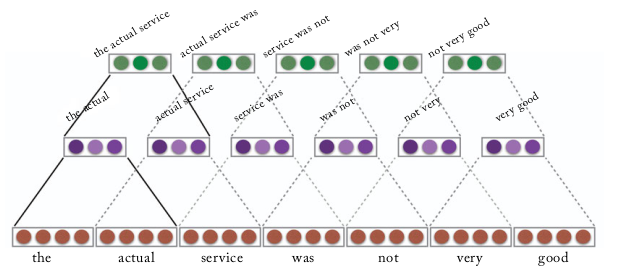
\includegraphics[keepaspectratio=true,scale=0.5]{figuras/cnnText}
	\caption[Aplicação de CNN em texto]{Aplicação de CNN em texto. Fonte: \citeonline[Página 160]{goldberg_neural_2017}}
	\label{fig:filterCnnText}
\end{figure}

Considera-se uma sentença $x_{1:n} = x_{1}, x_{2}, ..., x_{n}$ e um filtro $w$ que pode ser aplicado a intervalo de $h$ palavras. Através da operação de convolução é possível gerar uma nova característica, dada pela aplicação de uma função de ativação $g$ \cite{kim_convolutional_2014}:

\begin{equation}
	\label{eq:convolutionText}
	c_{i} = g(w \cdot x_{i:i+h-1} + b)
\end{equation}

Na Figura \ref{fig:filterCnnText}, é apresentado graficamente o processo da aplicação de filtros de convolução, seguidos da operação de junção em 2 camadas. A partir da Equação \ref{eq:convolutionText}, gera-se um novo conjunto de características extraídas do texto. Após isso, utiliza-se de uma camada de \textit{max pooling} para obter o maior valor daquele novo sub conjunto \cite{kim_convolutional_2014}.

$$c = [ c_{1}, c_{2}, ..., c_{n-h+1} ]$$
\begin{equation}
	\hat{c} = 
    \begin{cases}
    	maior(c) \\
        media(c) \\
        k-maiores(c) 
    \end{cases}
\end{equation}

O resultado de $\hat{c}$, é o maior valor significativo para o filtro $w$ aplicado sobre uma sentença entrada $x$. Em uma rede convolucional, tem-se vários filtros que possibilitam processar \cite{kim_convolutional_2014} e identificar os n-gramas mais importantes \cite{goldberg_neural_2017} dos corpos textuais.



\subsubsection{Redes recorrentes}

As redes neurais recorrentes possibilitam capturar características sequenciais dos dados. Sendo capaz de receber um vetor de entrada com tamanho variado e entregar um tamanho fixo na camada de saída \cite{goldberg_neural_2017}.

Dado um vetor $x_{1:n} = x_{1}, x_{2}, ..., x_{n}$ de entrada na $f(x_{i:n})$, será retornado um vetor $\hat{y}_{1:m} = \hat{y}_{1}, \hat{y}_{2}, ..., \hat{y}_{m}$, com o valor de $m$ fixado. Há um vetor de estados $s$ que carrega a informação do processamento dos neurônios anteriores. Uma rede neural recorrente é recursiva, pois o neurônio $i$, realizará o seguinte processamento $s_{i} = RNN_{i}(x_{i}, s_{i-1})$ \cite{mikolov_recurrent_2010}.

Na figura \ref{fig:rnnText}, as funções de $R, O$ em cada perceptron são, respectivamente, as funções $f$ e $g$ da equação \ref{eq:recorrentText}. O $\theta$, são os valores de hiperparametrização da rede.

\begin{figure}[ht]
	\centering
	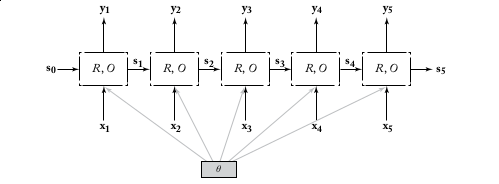
\includegraphics[keepaspectratio=true,scale=0.8]{figuras/rnnText}
	\caption[Arquitetura recursiva da RNN]{Arquitetura recursiva da RNN. Fonte: \citeonline[Página 166]{goldberg_neural_2017}}
	\label{fig:rnnText}
\end{figure}

Para utilizar a RNN como método de classificação, deve-se aplicar uma função de ativação $g$. Na equação \ref{eq:recorrentText}, tem-se também a função $f$, que é uma função de ativação responsável por juntar o vetor de estado $s_{i}$ com o vetor de entrada $x_{i}$ \cite{mikolov_recurrent_2010}.

\begin{equation}
	\label{eq:recorrentText}
	s_{i} = 
    \begin{cases}
    	i = 0 & f(S, x_{i}) \\
        i \neq 0 & f(s_{i-1}, x_{i})
    \end{cases}
\end{equation}
\begin{equation*}
	\hat{y_{i}} = g(s_{i})
\end{equation*}

Na Equação \ref{eq:recorrentText}, o valor de $S$ representa um hiper-parâmetro para a rede neural. Este é iniciado com um vetor de zeros $[0, 0, ..., 0]$.

\subsection{Métodos de avaliação}

A seguir serão apresentados o método de validação cruzada para modelos de classificação e as métricas para determinar o desempenho.

\subsubsection{Validação cruzada}

Para realizar a validação do modelo de classificação, há o modelo de validação cruzada. Este consiste em dividir o conjunto de dados em validação (30\%) e treino (70\%). A Figura \ref{fig:crossValidation} apresenta o processo para realizar a validação de um modelo classificador \cite{brink_real-world_2015}.

\begin{figure}[ht]
	\centering
    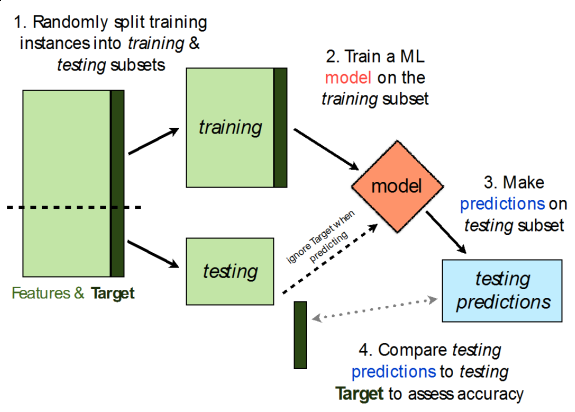
\includegraphics[keepaspectratio=true,scale=0.7]{figuras/crossValidation}
	\caption[Validação cruzada de modelos]{Validação cruzada de modelos. Fonte: \citeonline[Página 82]{brink_real-world_2015}}
	\label{fig:crossValidation}
\end{figure}

De acordo com \citeauthor{brink_real-world_2015} (\citeyear{brink_real-world_2015}), os passos para a validação são: 
\begin{enumerate}
	\item Realizar a divisão dos dados em conjunto de treino e teste.
	\item Utilizar o conjunto de treino para a construção do modelo.
    \item Utilizar o modelo para predizer o conjunto de dados de teste.
    \item Comparar os resultados da predição com os rótulos da base de teste e gerar as métricas.
\end{enumerate}

\subsubsection{Métricas}

Em modelos de classificação, é possível determinar com exatidão o resultado esperado em categorias. Com isso, é possível determinar o Verdadeiro Positivo, Verdadeiro Negativo que é quando o modelo acerta a predição. Para quando ele erra, há o Falso Positivo e Falso Negativo \cite{brink_real-world_2015}.

A Tabela \ref{tab:confusion} mostra a relação de Verdadeiros/Falsos Positivos/Negativos quando há mais de uma classe.

\begin{table}[ht]
	\centering    
	\caption{Matriz de confusão}
    \label{tab:confusion}
	\begin{tabular}{|c|c|c|c|c|}
      \hline
      Classe (N) & A & B & C & \\ \hline
      A & VP\textsubscript{A}  & eB\textsubscript{A} & eC\textsubscript{A} & T\textsubscript{A} \\ \hline
      B & eA\textsubscript{B}  & VP\textsubscript{B} & eC & T\textsubscript{B} \\ \hline
      C & eA\textsubscript{C}  & eB\textsubscript{C} & VP\textsubscript{C} & T\textsubscript{C} \\ \hline
       & P\textsubscript{A}  & P\textsubscript{B} & P\textsubscript{C} & \begin{tabular}[c]{@{}c@{}}
       							T = T\textsubscript{A} + T\textsubscript{B} + T\textsubscript{C}  \\ 
                                = P\textsubscript{A} + P\textsubscript{B} + P\textsubscript{C} 
       						\end{tabular} \\ \hline
    \end{tabular}\par Fonte: elaboração própria.
\end{table}

Os valores de eA\textsubscript{N}, eB\textsubscript{N} e eC\textsubscript{N} representam erros na predição, enquanto que os de VP\textsubscript{A}, VP\textsubscript{B} e VP\textsubscript{C}, os acertos. Ao somar-se os valores da coluna A na Tabela \ref{tab:confusion}, tem-se o resultado do VP\textsubscript{A} + eA\textsubscript{B} + eA\textsubscript{C}. Isso indica o quanto o modelo está predizendo a classe A. Ao mesmo tempo que somando-se a linha A, tem-se VP\textsubscript{A} + eB\textsubscript{A} + eC\textsubscript{A}, a qual representa o total de valores de A.

Com esta tabela, é possível obter valores numéricos para as métricas de acurácia (ou eficiência), revocação (ou sensibilidade), taxa de verdadeiros negativos, taxa de falsos positivos e negativos, precisão. Além de outras métricas que utilizam estas para seus cálculos \cite{rodriguez_quality_2016}.

As métricas a seguir serão utilizadas a fim de validar a qualidade e evolução de performance dos modelos. Todas as métricas a seguir são descritas por \citeauthor{rodriguez_quality_2016} (\citeyear{rodriguez_quality_2016}):

\begin{description}
	\item Revocação: trata-se da taxa de acertos para a classe N. A fórmula é: $R = \frac{VP_{N}}{T\textsubscript{N}}$.
    \item Precisão: também conhecido como "acurácia da classe N", representa a proporção de VP para os valores preditos em N. $P = \frac{VP_{N}}{P\textsubscript{N}}$
    \item Taxa geral de acerto: também conhecido como "acurácia do modelo", representa o quanto ele acerta de todas as classes. $G = \frac{\sum{VP_{N}}}{T}$
\end{description}

A revocação e precisão são para analisar pontualmente o comportamento do modelo com cada classe. Enquanto que a taxa geral de acerto irá proporcionar a informação da capacidade do modelo em aprender como separar as peças. Além disso, a matriz de confusão (Tabela \ref{tab:confusion}) será utilizada para verificar quais classes são mais confundidas pelo modelo.

\section{Sistema Jurídico Brasileiro}

A estrutura do sistema jurídico brasileiro é estabelecida pela Constituição Federal de 1988. Ela prevê quais são os órgãos que compõem o Poder Judiciário, as competências que eles possuem, onde estão localizados, o tamanho dos representantes das instâncias superiores e como se faz a investidura aos cargos \cite{brasil_constituicao_1988}. Além da Constituição, para um estudo mais completo, são necessárias as Lei n.º 8.457/1992, que estabelece a primeira instância da Justiça Militar \cite{noauthor_lei_1992} e a n.º 12.665/2012, a qual define as Turmas Recursais para segunda instância de Juizados Especiais \cite{noauthor_lei_2012}.

Para ter um entendimento completo sobre as peças jurídicas e suas origens, é preciso ter conhecimento sobre como estão organizados os órgãos do Judiciário, pois são através deles que a população vivencia um processo \cite{amendoeira_jr_manual_2012}.

\begin{figure}[ht]
	\centering
    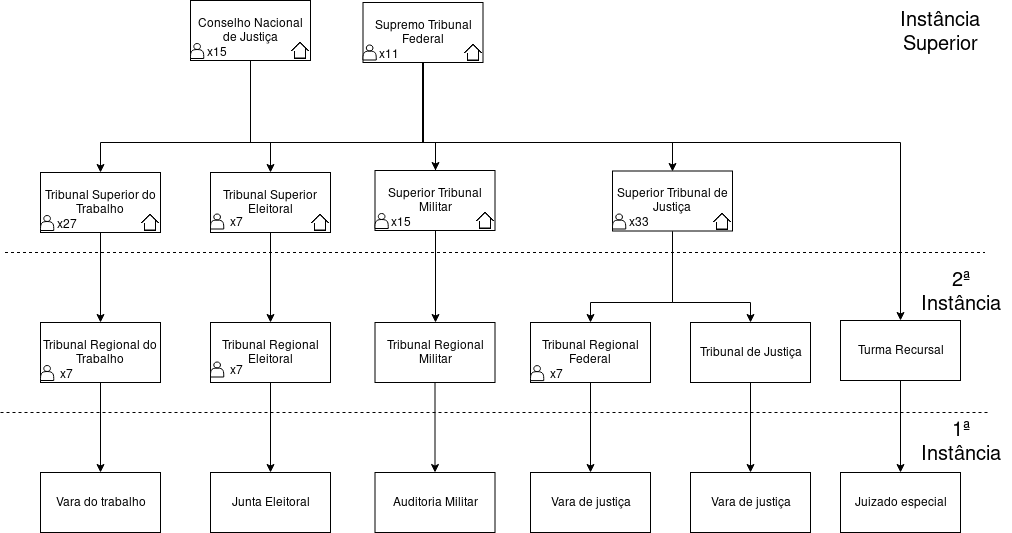
\includegraphics[keepaspectratio=true,scale=0.4]{figuras/sistemaJudiciario}
	\caption[Sistema judiciário]{Organização do sistema jurídico brasileiro. Fonte: elaboração própria}
	\label{fig:sistemaJudiciario}
\end{figure}

Para organizar melhor o trabalho do sistema judiciário, separou-se a justiça comum em algumas áreas para lidar com temas específicos: os assuntos trabalhistas, os eleitorais e uma especialização para lidar com as Leis Militares \cite{amendoeira_jr_manual_2012}. 

\subsection{Instância superior - Tribunais Superiores e STF}

Como apresentado na Figura \ref{fig:sistemaJudiciario}, são tribunais superiores Supremo Tribunal Federal, Superior Tribunal de Justiça (STJ), Tribunal Superior Eleitoral (TSE), Tribunal Superior do Trabalho (TST) e Superior Tribunal Militar (STM) \cite{brasil_constituicao_1988}.

O STF e o STJ não se encaixam em nenhuma das justiças comum ou especializadas. A função primordial do STF é o controle de constitucionalidade das Leis Federais em conformidade com a CF (\citeyear{brasil_constituicao_1988}) e a do STJ é o controle de legalidade das Leis do Brasil em conformidade com as Leis Federais \cite{brasil_constituicao_1988}.
Eles não são chamados de terceira instância devido ao princípio da dupla jurisdição. A correta denominação é instância superior, pois em Recurso Extraordinário, julgam as teses jurídicas e não os fatos do processo \cite{amendoeira_jr_manual_2012}.

Os tribunais TST, TSE e STM compõe também a instância superior, mas estes julgam apenas os recursos de sua área de especialização na justiça \cite{brasil_constituicao_1988}.

Todos possuem sua sede na capital do Brasil e o número mínimo de representantes está estabelecido diretamente na CF (\citeyear{brasil_constituicao_1988}). Na Figura \ref{fig:sistemaJudiciario}, são representados estes valores para cada um deles. Estes Tribunais também possuem a competência para estabelecer o número de servidores nas instâncias inferiores \cite{brasil_constituicao_1988}.

\subsection{2ª instância - Tribunais}

Além dos Tribunais de segunda instância da justiça especial: o Tribunal Regional Eleitoral, o Tribunal Regional do Trabalho e o Tribunal Regional Militar, tem-se os Tribunais que compõe a justiça comum o Tribunal Regional Federal e os Tribunais Estaduais de Justiça \cite{brasil_constituicao_1988}. Há também as Turmas Recursais que representam a Segunda Instância para os juizados especiais \cite{noauthor_lei_2012}.

Nestes Tribunais, julgam-se os Recursos Ordinários, as provas, as evidências, diferentemente dos Tribunais de instância superior \cite{amendoeira_jr_manual_2012}.

\subsection{1ª instância}

Para se entender a organização da justiça de primeira instância, é preciso definir como estão estruturadas a separação da jurisdição dos Tribunais.

Cada Estado e o Distrito Federal dividem-se em comarcas (ou foros), no qual cada um destes possue uma ou mais varas especializadas  para as justiças comum e do trabalho \cite{amendoeira_jr_manual_2012}. Para a Justiça Militar, o território nacional está separado em circunscrições, onde cada uma possui sua Auditoria Militar \cite{noauthor_lei_1992}. Já para a Justiça Eleitoral, existem juntas eleitorais que subdividem os Estados e o Distrito Federal em zonas distintas \cite{brasil_constituicao_1988}.

A seguir são apresentadas as definições:

\begin{description}
	\item \textbf{Circunscrição} é uma divisão geográfica administrativa para restringir a atuação de um tribunal \cite[p. 71]{guimaraes_dicionario_2012}.
	\item \textbf{Comarca} é uma circunscrição sob jurisdição de juízes, na qual o território esta subdividido \cite[p. 75]{guimaraes_dicionario_2012}.
    \item \textbf{Vara} é uma repartição judiciária com seu domínio a cargo de um juiz \cite[p. 259]{guimaraes_dicionario_2012}.
\end{description}


\section{Código Processual Civil (CPC)}
\label{sec:cpc}

O CPC (Lei n.º 13.105/2015) é a lei que define como devem ser estruturados os processos civis. Ele é o meio pelo qual o juiz concretiza as leis, considerando os interesses entre as partes envolvidas.

O processo civil possui duas categorias de procedimentos adotados: o comum e especial. Neste trabalho tratar-se-á apenas do comum. A seguir, será apresentado para o entendimento das peças jurídicas avaliadas pelo STF, suas características em meio ao processo civil.

\begin{figure}[ht]
	\centering
    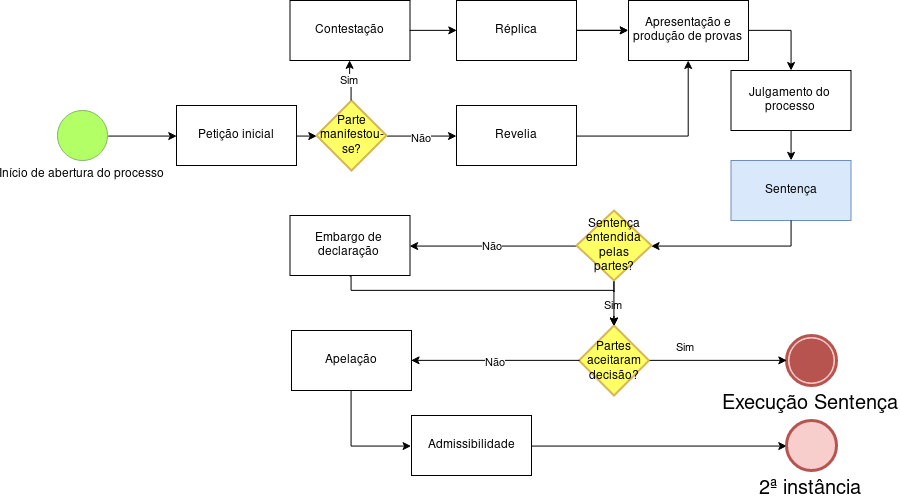
\includegraphics[keepaspectratio=true,scale=0.4]{figuras/processoPrimeira}
	\caption[Processo judiciário - 1ª Instância]{Processo judiciário - 1ª Instância. Fonte: elaboração própria}
	\label{fig:processoPrimeira}
\end{figure}

\subsection{1ª instância}

O processo civil dá-se início por meio de uma peça chama de Petição Inicial. E através deles, a parte faz seus pedidos ao juiz e identifica quem é a outra parte, que por sua vez, possui o direito de se manifestar ou não \cite{brasil_lei_2015}. Chama-se esta fase de postulatória \cite{goncalves_direito_2016}.

A etapa seguinte é a ordinatória, caracterizada pelo direito de réplica. Depois disso, inicia-se a fase instrutória caracterizada pela produção de provas \cite{goncalves_direito_2016}.

A etapa decisória tem o ato da sentença \cite{goncalves_direito_2016}. Deste, é gerada a peça que descreve a decisão tomada pelo juiz mediante os fatos apresentados pelas partes. Uma Sentença é inalterável pelo próprio juiz que a proferiu, poderá apenas ser esclarecida pelo recurso de Embargo de Declaração \cite{brasil_lei_2015}.

Após a sentença, as partes têm o direito garantido pelo duplo grau de jurisdição de realizar a apelação. O processo será enviado a um órgão segunda instância caso esteja em conformidade com a lei \cite{goncalves_direito_2016}.

O Artigo n.º 489 do CPC (Lei n.º 13.105/2015) define que existem em todas as sentenças três elementos fundamentais:

\begin{citacao}
I - o relatório, que conterá os nomes das partes, a identificação do caso, com a suma do pedido e da contestação, e o registro das principais ocorrências havidas no andamento do processo;

II - os fundamentos, em que o juiz analisará as questões de fato e de direito;

III - o dispositivo, em que o juiz resolverá as questões principais que as partes lhe submeterem. \citeonline{brasil_lei_2015}
\end{citacao}

\subsection{2ª Instância}

Garantido pelo princípio da dupla jurisdição, os processos que cumprem com os requisitos formais de uma apelação são direcionados ao Tribunal de segunda instância competente para sua análise. Um Acórdão é o resultado do voto de três ou mais desembargadores, a decisão que mais receber votos é a final, portanto deve ser ímpar o número de juízes na sessão. 

Após essa fase decisória, há o momento para as partes ou o Ministério Público elaborarem os recursos. Na Figura \ref{fig:processoSegunda}, são as atividades do fluxo, após o procedimento de primeira instância.

\begin{figure}[ht]
	\centering
    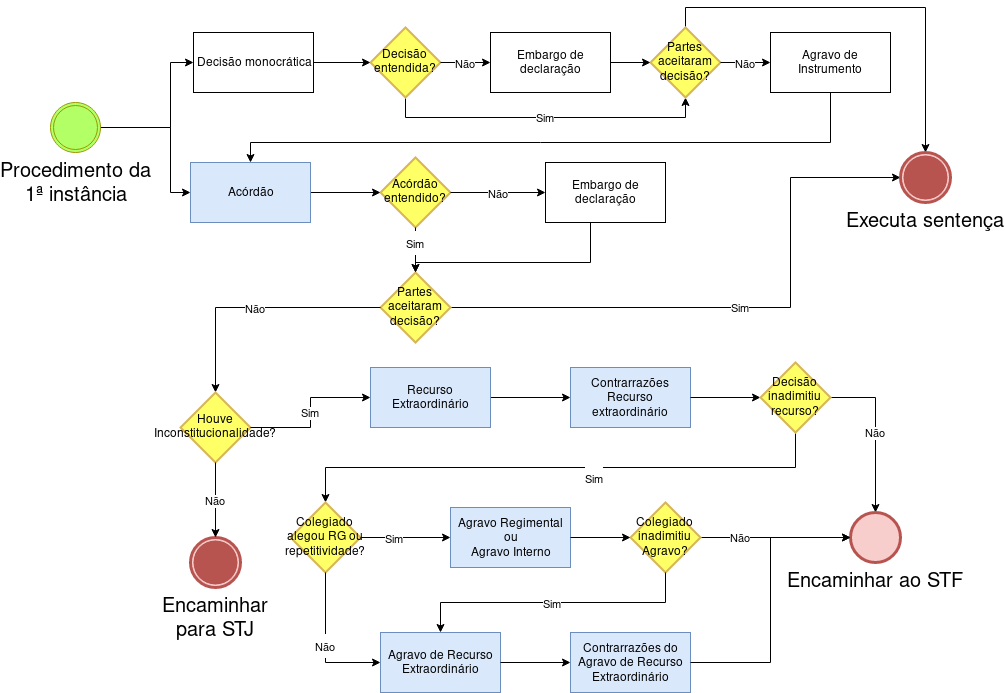
\includegraphics[keepaspectratio=true,scale=0.4]{figuras/processoSegunda}
	\caption[Processo judiciário - 2ª Instância]{Processo judiciário - 2ª Instância. Fonte: elaboração própria}
	\label{fig:processoSegunda}
\end{figure}

O Agravo Interno ou Regimental, deve ter em seu conteúdo apenas a informação sobre a questão agravada e encaminhado diretamente ao tribunal competente.

Para Recurso Extraordinário (RE), este deve ser apresentado ao Presidente ou Vice-Presidente do Tribunal em que foi recorrida a decisão. O RE deve conter as informações sobre as razões do pedido, a exposição do quê ocorreu associado a regra do direito e discorrer sobre a validade da interposição do recurso. Quando houver recursos simultâneos ao STJ e STF, o processo deve, primeiramente, ser encaminhado ao STJ \cite{brasil_lei_2015}.

As características procedurais de um Agravo em Recurso Extraordinário (ARE) são iguais às de um RE. A distinção entre ambas as peças são seus conteúdos, no qual o RE será relacionado a alguma inconstitucionalidade e o ARE será um contraponto à inadmissão do recurso.

\subsection{Instância superior e o Supremo Tribunal Federal}

A decisão proferida pelos ministros do STF sobre a Repercussão Geral (RG) são irrecorríveis. Caso haja RG, ou seja, ele cumpre os requisitos do § 1º do Artigo n.º 1.035 do CPC (Lei n.º 13.105/2015)
"Para efeito de repercussão geral, será considerada a existência ou não de questões relevantes do ponto de vista econômico, político, social ou jurídico que ultrapassem os interesses subjetivos do processo"\ - \citeonline{brasil_lei_2015} o processo é distribuído para que os Ministros do Tribunal possam julgar a questão do RE. 

\begin{figure}[ht]
	\centering
    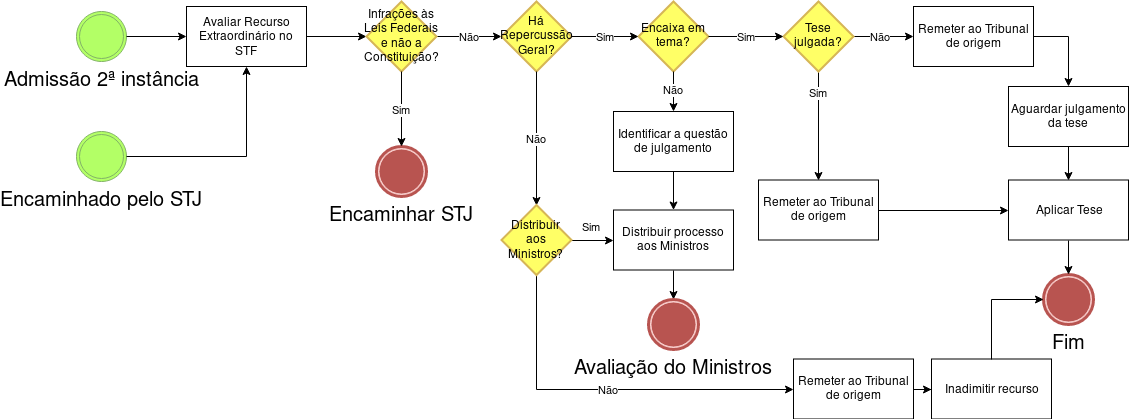
\includegraphics[keepaspectratio=true,scale=0.4]{figuras/processoSuperior}
	\caption[Processo judiciário - Instância Superior]{Processo judiciário - Instância Superior e STF. Fonte: elaboração própria}
	\label{fig:processoSuperior}
\end{figure}

Na figura \ref{fig:processoSuperior}, a atividade de Avaliação dos Ministros é composta por um outro conjunto de atividades descritas no Regimento Interno do STF \cite{noauthor_regimento_2016} e na Constituição Federal (\citeyear{brasil_constituicao_1988}). 

Existem outras atividades desenvolvidas pelo STF que não foram apresentadas na Figura \ref{fig:processoSuperior}. Estas atividades estão relacionadas ao Regimento Interno \cite{noauthor_regimento_2016} deste Tribunal e o que eles fazem com as peças. Ou seja, não há produção de novos documentos internamente os quais sejam analisados para definir se há ou não Repercussão Geral.